% !TEX root = ../main.tex

\section{Bindings for emlib}
\label{sub:interfacing_with_emlib}

The \gls{ffi} available in {\rust} has been used to interface with Silabs' emlib.
This way, we have been able to create thin wrappers around the \gls{api} for the different peripherals that we have used in the project, without porting the core logic itself.
The following sections explains the process of defining and implementing the \gls{ffi} in {\rust} that is used to access and control the peripherals on the {\gecko}.
We will start by showing an example of what it is like to use Silab's emlib (with C), and then move on to what it looks like to use the bindings in {\rust}.

\subsection{Defining the Bindings}

The \code{Timer} peripheral \cite{an0014_timer} works as a good example to demonstrate what the {\rust} bindings look like.
The module is fairly small, it mostly exposes functions to set up and initialize four different timers that can be used for up, down, up/down, and input- and output-capture.
The program shown in \autoref{lst:timer_program_c} is an example of initializing the \code{Timer0} peripheral on the {\gecko}, note that this is not a complete working example, it only shows the most important parts required to use the Timer module.
First, in order to use a peripheral, its clock need to be enabled.
Every external clock are disabled by default \todo{Is this true? Is every clock disabled?} in order for the peripherals not to draw any power, by enabling the clock the \gls{mcu} will get access to control it.
Then an initialization structure for the Timer module is acquired, this structure has fields to configure many different properties of the Timer, in the same way as described in \autoref{ssec:memory_mapped_io}.

\begin{listing}[h]
\begin{minted}{c}
// Enable clock for TIMER0 module
CMU_ClockEnable(cmuClock_TIMER0, true);
// Select TIMER0 parameters
TIMER_Init_TypeDef timerInit = TIMER_INIT_DEFAULT;
// Enable overflow interrupt
TIMER_IntEnable(TIMER0, TIMER_IF_OF);
// Enable TIMER0 interrupt vector in NVIC
NVIC_EnableIRQ(TIMER0_IRQn);
// Set TIMER Top value
TIMER_TopSet(TIMER0, TOP);
// Configure TIMER
TIMER_Init(TIMER0, &timerInit);
\end{minted}
\caption{Initializing a Timer in C}
\label{lst:timer_program_c}
\end{listing}

The next lines enables interrupts for the Timer, and the NVIC interrupt vector is set up to call the function shown in \autoref{lst:timer_interrupt_handler} every time an interrupt it triggered by the Timer.
All this function does is to clear the interrupt signal and toggle the value of an LED.
We can imagine an application where the Timer is configured to trigger an interrupt every minute to toggle the LED, and in between the interrupts the \gls{mcu} can be put to sleep in order to save power.
Interrupts like this are an important part of programming the {\gecko}.
They can be used for an asynchronous programming model where the application is defined by the code in the different interrupt handlers, and like in the example above, the \gls{mcu} can be put to sleep in between interrupts.

\begin{listing}[h]
\begin{minted}{c}
void TIMER0_IRQHandler(void) {
  // Clear flag for TIMER0 overflow interrupt
  TIMER_IntClear(TIMER0, TIMER_IF_OF);
  // Toggle LED ON/OFF
  GPIO_PinOutToggle(LED_PORT, LED_PIN);
}
\end{minted}
\caption{Timer Interrupt Handler}
\label{lst:timer_interrupt_handler}
\end{listing}

The equivalent program written in {\rust} is shown in \autoref{lst:timer_program_rust}.
Semantically they are the same, but the usage differs slightly, which is natural since we are using a higher level programming language.
Instead of calling functions that are included through a {\C} header file, we are calling functions that are available through a {\rust} module.
For example, the \code{Clock} enum is part of the \code{cmu} module, and the \func{enable\_irq} function is part of the \code{nvic} module.
This modularization of peripherals can help to make the code less verbose by partially including modules.
It is also worth to notice the difference between how the \code{Timer0} structure can be treated like an object with its own member methods in {\rust}, instead of being passed as the first parameter to every function that requires it, like in {\C}.

\begin{listing}[h]
\begin{minted}{rust}
// Enable clock for TIMER0 module
cmu::clock_enable(cmu::Clock::TIMER0, true);
// Select TIMER0 parameters
let timer_init = Default::default();
// Enable overflow interrupt
let timer0 = timer::Timer::timer0();
timer0.int_enable(timer::TIMER_IF_OF);
// Enable TIMER0 interrupt vector in NVIC
nvic::enable_irq(nvic::IRQn::TIMER0);
// Set TIMER Top value
timer0.top_set(TOP);
// Configure TIMER
timer0.init(&timer_init);
\end{minted}
\caption{Initializing a Timer in {\rust}}
\label{lst:timer_program_rust}
\end{listing}

\subsection{Exposing Static Inline Functions to Rrust}

In order to work with structures and enums originally defined in C, we had to redefine them in {\rust} and mark them with \attrib{\#[repr(C)]} so that {\rust} can guarantee that the data-elements are {\C} compatible.
The header files in the peripheral \gls{api} also defines many functions as \code{static inline}, which only make the functions accessible by including the header file.
Since it is not possible to include {\C} header files directly in {\rust}, we had to expose these functions through one extra layer of {\C} code.
As an example, the \func{TIMER\_IntEnable} function is defined as \code{static inline} in \file{em\_timer.h}, in order to call this function through {\rust} we had to expose it through the file \file{timer.c}, as shown in \autoref{lst:exposing_static_inline}.

\begin{listing}[h]
\begin{minted}{c}
#include "en_timer.h"

void STATIC_INLINE_TIMER_IntEnable(TIMER_TypeDef *timer,
                                   uint32_t flags) {
    TIMER_IntEnable(timer, flags);
}
\end{minted}
\caption{Exposing a \code{static inline} function to {\rust}.}
\label{lst:exposing_static_inline}
\end{listing}

In the {\rust} module definition of Timer, the function has to be made available through the \code{extern} block shown in \autoref{lst:rust_ffi_example}.
As described in \autoref{ssub:unsafe_code}, every function available through the \gls{ffi} are considered {\unsafe} because {\rust} knows nothing about the function, other than its parameters and its return value.
Thus, in order to make it practical to use the library in a seemingly safe manner, we wrap the calls to the foreign functions in an {\unsafe} block, in the respective function defined in {\rust}.

\begin{listing}[h]
\begin{minted}{rust}
impl Timer {
    pub fn int_enable(&self, flags: u32) {
        unsafe { STATIC_INLINE_TIMER_IntEnable(self, flags)}
    }
}

extern {
    fn STATIC_INLINE_TIMER_IntEnable(timer: &Timer, flags: u32);
}
\end{minted}
\caption{Defining and using a function through the {\rust} \gls{ffi}.}
\label{lst:rust_ffi_example}
\end{listing}

If we compare the call-stacks between calling the \code{timer0.int\_enable} function in {\rust} and calling the \func{TIMER\_IntEnable} function in C, we can see that every function call through the \gls{ffi} requires \emph{two} extra function calls.
These are simple wrappers which require extra unconditional jumps in the code, and performance-wise it is a very unnecessary overhead to have one to two extra stack frames allocated for \emph{every} function call through the \gls{ffi}.
By compiling the code with optimization, {\rust} will get rid of the overhead introduced by the function that wraps around the call to the foreign function.
Additionally, by enabling \concept{link-time-optimizations} during the compilations, LLVM will remove the overhead entirely, which results in the same performance and similar call-stacks between {\C} and {\rust}.
This is a working example of one of {\rust}'s many zero-cost abstractions.

\subsection{Naming Conventions}

We have tried to keep \emlib's naming convention across the layer of bindings.
This makes it easy for anyone reading either the C- or the {\rust}-code to translate and understand the code between the two languages.
Since every constant, enum-field, or struct-name is directly accessible by name in C, if the corresponding header file is included, it is important that names of such fields can be separated from each other and do not cause a naming collision.

\begin{listing}[h]
\begin{minted}{c}
typedef enum {
  timerCCModeOff     = _TIMER_CC_CTRL_MODE_OFF,
  timerCCModeCapture = _TIMER_CC_CTRL_MODE_INPUTCAPTURE,
  // ...
} TIMER_CCMode_TypeDef;
\end{minted}
\caption{Part of a Timer enum defined in C.}
\label{lst:enum_naming_c}
\end{listing}

As an example, two fields of an enum from \file{em\_timer.h} is shown in \autoref{lst:enum_naming_c}.
From each field in the enum we can extract 1) its module name \file{timer}, 2) its typedef name \code{CCMode} and 3) its field name \code{Off} or \code{Capture}.
\rust allows us to keep the same naming convention at the same time as utilizing its modularity.
\autoref{lst:enum_naming_rust} shows the enum ported to {\rust}, where both the module name and the typedef name has been left out, and only the field names have remained.
However, the naming convention remains the same when the fields are used, e.g. the expression ``\code{let mode = timer::CCMode::Capture;}'' in {\rust} shows the similarity with the equivalent expression in C: ``\code{int mode = timerCCModeCapture;}''.

\begin{listing}[h]
\begin{minted}{rust}
pub enum CCMode {
  Off     = _TIMER_CC_CTRL_MODE_OFF,
  Capture = _TIMER_CC_CTRL_MODE_INPUTCAPTURE,
  // ...
}
\end{minted}
\caption{The enum ported to {\rust}.}
\label{lst:enum_naming_rust}
\end{listing}

\subsection{Testing}
\label{ssub:testing}

This section describes a small Unit testing framework developed for testing the emlib bindings.

\subsubsection{Why Unit testing}

Early on in the development phase of the emlib bindings we saw the need for a testing framework.
This was provoked by the fact that testing on an embedded system is a time consuming and tedious task.
More often than not you find your self running the code in the debugger inspecting the call stack and arguments to ensure that the bindings are calling the correct functions with the correct arguments.
The fact about arguments has a subtle point to it.

We are working in two statically typed languages here which leads to the compiler statically assuring that the correct types are passed around, but at the language boundries there are no checks for assuring that the memory layout of the datatypes in C and Rust match.
Currently the Rust FFI requires the programmer to redefine the datatypes like structs and enums on the Rust side in order to call into C functions that takes these datatypes as arguments.
This process proved to be too error prone and time consuming to verify manually.

\subsubsection{Framework}

To meet this problem, a featherweight testing framework was developed which enabled this verification to be automated.
The goal of the framework was to initialize the data on the Rust side execute the \gls{ffi} and verify the correct function where called with the exact data as supplied.
To do this we set up a framework to replace the emlib code with statically generated test mocks, execute test cases where the datastructures where setup in Rust code and then verify the correctness in C code.
All of this was executed on the \textbf{Gecko} which reported test failure/success over Uart.

The framework implemented is a small test runner utilizing CMock \cite{web:cmock} and Unity \cite{web:unity} for mocking and assertions respectivly.

An test case for verifying that the \texttt{ADC\_Init} with default argument is working properly is given in \autoref{lst:test:adc}.


\begin{listing}[H]
  \centering
  \begin{minipage}{\textwidth}
  \begin{listing}
    \begin{minted}{rust}
fn test_init_called_with_default() {
  // FFI call to the C function below
  unsafe { adc_expect_init_called_with_default(); }

  let adc0 = adc::Adc::adc0();
  // Call the emlib bindings with an default argument
  adc0.init(&Default::default());
}
    \end{minted}
    \label{lst:test:adc:rust}
    \caption{Rust side of ADC\_Init test}
  \end{listing}
  \end{minipage}

  \begin{minipage}{\textwidth}
  \begin{listing}
    \begin{minted}{c}
void adc_expect_init_called_with_default() {
  static ADC_Init_TypeDef init = ADC_INIT_DEFAULT;
  // setup the expected value on the Mock
  ADC_Init_Expect(ADC0, &init);
}
    \end{minted}
    \label{lst:test:adc:c}
    \caption{C side of ADC\_Init test}
  \end{listing}
  \end{minipage}

  \caption{Test case for ADC\_Init with default values}
  \label{lst:test:adc}
\end{listing}

When using mocking in unit tests the workflow of for the user seems reversed compared to standard unit tests.
First you setup the expected results with by calling the \texttt{ADC\_Init\_Expect} function on the mock as shown in \auroref{lst:test:adc:c}.
This method is in fact called through \gls{ffi} right at the top of the test case in \autoref{lst:test:adc:rust}.
When the expected result is setup the test case goes on to create an \gls{adc} object using the Rust bindings and calling the \texttt{init} function causing the \gls{ffi} library bindings to be executed.
When the test returns, the test runner is responsible for calling a \texttt{Verify} function on the mock object.
This function causes the program to fail and report status over Uart if the expectation set up was not met.

\autoref{fig:test-framework} shows a diagram of the flow between \textit{Test Runner}, \textit{Test Case}, \textit{emlib Bindings} as \gls{CUT} and the \textit{emlib Mock} when executing the testcase above.

\begin{figure}[H]
  \begin{center}
    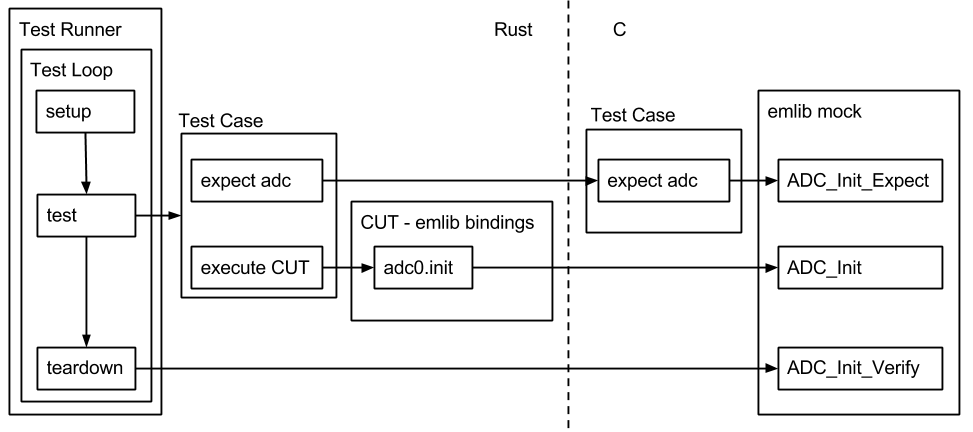
\includegraphics[scale=0.3]{figures/testframework}
  \end{center}
  \caption{Flowchart for test framework}
  \label{fig:test-framework}
\end{figure}

We see that the two boxes marked with \textit{Test Case} are the pieces of code the user of the framework, presented in \autoref{lst:test:adc}, writes.
The stippled vertical line shows the separation between Rust and C code, all the three calls which cross this line is implemented using the Rust \gls{ffi}.

\subsubsection{Rust libtest}

The Rust programming language contains a testing framework within the standard library.
The reasons for not using it to test the bindings is that we wanted to run the tests on the \textbf{Gecko}.
The rational for this is that the tests are mostly checking that the datatypes used on the Rust and C side of the bindings are compatible.
Therefore we need to use the proper compilers and compiler targets for the platform, verifying that the OSX platform gcc and rust compiler has compatible types does not help in this respect.
Consequently, given that the testing framework in the standard library relies heavily on the Rust standard library RSL as discussed in \autoref{sec:back:lib}, this renders the framework unusable for our embedded platform.

\subsection{Thoughts and Review}

\todo{Does it make sense to have this section here? Should content like this be mover somewhere else (like in the discussion chapter), or is this a good place?}

Writing the bindings for different the peripherals was a tedious work, that required careful review of the \emlib source code in order to correctly port enum- and struct-definitions from {\C} to {\rust}.
Additionally, we had to redefine many constants, like the names of memory-mapped register bit-fields like the ones presented earlier in \autoref{fig:back:memorymapped}, or values calculated from various {\C} macros defined in header files that are used throughout the library.
We had to retrieve the value of the constants by debugging the source code and explicitly look up the value of these constants if they were only implicitly defined in the header files.

Since we have constrained our library to only support the EFM32GG990 devices we chose to manually write the bindings for the library, instead of generating the bindings through some kind of automated process.
There were already a couple of tools available for generating such C-bindings automatically, that could possibly have made the process quicker.
However, we chose not to utilize such tools because of the reasons described below.

\begin{itemize}
    \item It was quick and easy to get started with code for a new peripheral.
    This argument was especially important when the project started out, because we still had no clue of how the project would evolve and what it was going to look like.

    \item It was an advantage to depend on as few third party tools as possible, since both {\rust} and all available libraries would be unstable until the 1.0 release of the language.

    \item We wanted to keep the naming convention of our bindings as similar to \emlib as possible, this would not have been easy to keep consistent with an automated process, partly because there are exceptions where these conventions do not fully hold.
    It is however an interesting problem that would have a higher priority if the library were ever to support more than one EFM32 device.

    \item We could focus on writing bindings for smaller parts of each module separately when we first needed them, which would split the work into smaller work-packages.
\end{itemize}
